\documentclass[border=2pt]{standalone}
\usepackage{xcolor}
\usepackage{pgfplots}
\pgfplotsset{compat=1.18}
\definecolor{red}{rgb}{0.7,0.11,0.11}
\definecolor{blue}{rgb}{0.0,0.20,0.42}
\definecolor{green}{rgb}{0.11,0.35,0.02}
\begin{document}
\definecolor{placeholderbg}{rgb}{1.00, 0.97, 0.78}
\pagecolor{placeholderbg}
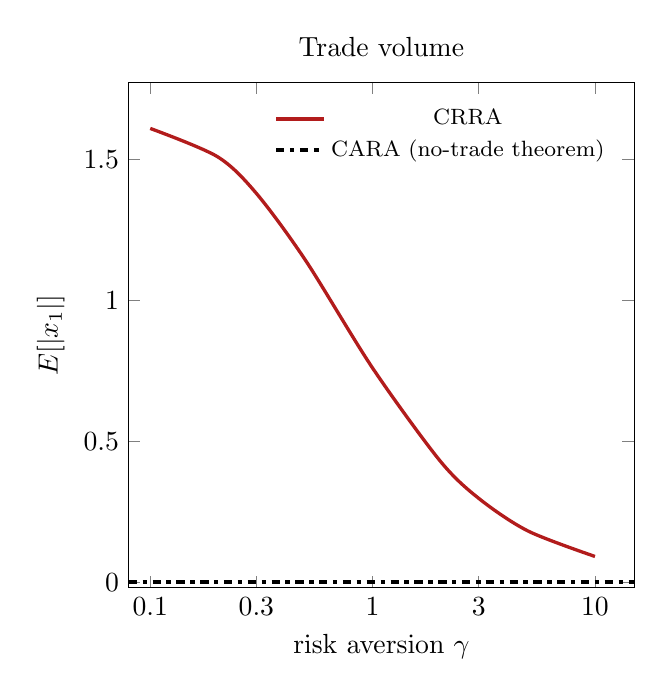
\begin{tikzpicture}
\begin{axis}[
    width=8cm, height=8cm,
    xmode=log,
    xmin=0.08, xmax=15,
    ymin=-0.02,
    xtick={0.1,0.3,1,3,10},
    xticklabels={0.1,0.3,1,3,10},
    xlabel={risk aversion $\gamma$},
    ylabel={$\mathbb{E}[|x_1|]$},
    title={Trade volume},
    legend pos=north east,
    legend style={fill=none, draw=none, font=\footnotesize},
    smooth,
]
\addplot[very thick, color=red, smooth]
    coordinates {(0.1000,1.609916) (0.2000,1.510289) (0.3000,1.379648) (0.5000,1.141275) (1.0000,0.759801) (2.0000,0.432851) (3.0000,0.297689) (5.0000,0.181743) (10.0000,0.091538)};
\addlegendentry{CRRA}
\addplot[ultra thick, color=black, dashdotted]
    coordinates {(0.08,0)(15,0)};
\addlegendentry{CARA (no-trade theorem)}
\end{axis}
\end{tikzpicture}
\end{document}
